\clearpage
\section{5 СРАВНЕНИЕ С КЛАССИЧЕСКОЙ РЕАЛИЗАЦИЕЙ}
В качестве тестового меша была использована модель Thai Statue из The Stanford 3D Scanning Repository~\cite{StanfordRepo}.

Для сравнения была написана вторая версия приложения отрисовки, использующая монолитные лоды.
Для указания версии используется определение макроса.

Для создания лодов был использован модификатор Decimate в Blender.
Размеры сгенерированных лодов приведены в таблице~\ref{tab:lod-sizes}.

\begin{table}[h]
    \centering

    \begin{tabular}{lrr}
        \hline \hline
        & Количество треугольников
        & Количество вершин \\ \hline
        LOD0 & 10 000 000 & 4 999 996 \\
        LOD1 &  1 000 000 &   499 996 \\
        LOD2 &    100 000 &    49 996 \\
        LOD3 &     10 000 &      4996 \\
        LOD4 &       1000 &       496 \\
        LOD5 &        100 &        46 \\
        LOD6 &         10 &        18 \\
        \hline \hline
    \end{tabular}

    \caption{Размеры лодов}
    \label{tab:lod-sizes}
\end{table}

При конвертации в граф мешлетов получен граф с характеристиками, указанными в таблице~\ref{tab:graph-sizes}.

\begin{table}[h]
    \centering

    \begin{tabular}{lr}
        \hline \hline
        Всего мешлетов    &    269 925 \\
        Истоков           &    104 167 \\
        Уникальных вершин &  6 166 095 \\
        Индексов          & 19 782 880 \\
        Всего примитивов  & 24 616 574 \\
        \hline \hline
    \end{tabular}

    \caption{Граф мешлетов}
    \label{tab:graph-sizes}
\end{table}

В процессе сравнения также была опробован метод отрисовки мешлетов без двойной индексации --- с разворачиванием массива вершин так, чтобы одному мешлету соответствовали записанные подряд в памяти вершины, а не записанные подряд в памяти индексы вершин.
При использовании вершин размером 24 байта и индексов размером 4 байта это даёт массив вершин размером 452.8 мегабайта (474~789~120 байт), в сравнении с суммарным размером массивов вершин и индексов в 216.6 мегабайт (227~117~800 байт), т.е. дополнительные 109\% потребляемой памяти.
Несмотря на это, подобный подход позволил увеличить производительность отрисовки, см. таблицу~\ref{tab:fps}.

Для замера производительности была настроена одинаковая сцена из 64 объектов с одинаковым исходным мешем, содержащим 10 млн. треугольников.
Для замеров приложение было запущено в полноэкранном режиме.

Замеры выполнялись на ноутбуке с 16 ГБ оперативной памяти, видеокартой NVidia GeForce RTX 3060 Laptop GPU, процессором AMD Ryzen 7 5800H (3201 МГц, 8 физических ядер, 16 логических процессоров), разрешением монитора 2560 на 1440 и частотой обновления 165 Гц.

Было измерено количество кадров в секунду (FPS), количество отправляемых на растеризацию примитивов, количество растеризуемых примитивов и количество вызовов пиксельного шейдера.

Скриншоты выполнения приведены на рисунках \ref{fig:impl-lod0}, \ref{fig:impl-cluster-1}, \ref{fig:impl-cluster-2} и~\ref{fig:impl-mono}.
Результаты измерений приведены в таблице~\ref{tab:fps}.
На скриншотах не видно существенной разницы в сравнении с режимом отображения всех объектов в максимальной детализации, но заметно пятикратное увеличение производительности даже в худшей из полученных реализаций лодов.

\begin{figure}[H]
    \centering
    \includegraphics[width=\textwidth]{pics/comparison-0.png}
    \caption{Наивысшее разрешение, без лодов}
    \label{fig:impl-lod0}
\end{figure}

\begin{figure}[H]
    \centering
    \includegraphics[width=\textwidth]{pics/comparison-1.png}
    \caption{Кластерные лоды}
    \label{fig:impl-cluster-1}
\end{figure}

\begin{figure}[H]
    \centering
    \includegraphics[width=\textwidth]{pics/comparison-2.png}
    \caption{Кластерные лоды, без массива индексов}
    \label{fig:impl-cluster-2}
\end{figure}

\begin{figure}[H]
    \centering
    \includegraphics[width=\textwidth]{pics/comparison-3.png}
    \caption{Монолитные лоды}
    \label{fig:impl-mono}
\end{figure}

\begin{table}[h]
    \centering
    \begin{tabular}{lrrrr}
        \hline \hline
        Тип отрисовки
        & FPS
        & Отправлено
        & Растеризовано
        & Пикселей \\ \hline
        Наивысшее разрешение
        & 5.3
        & 640 000 000
        & 631 812 157
        & 2 473 141 \\
        Монолитные лоды
        & \textbf{117.8}
        & 28 900 000
        & 22 478 691
        & 2 473 397 \\
        Кластерные лоды
        & 27.2
        & 56 021 881
        & 55 940 686
        & 2 492 760 \\
        \makecell[l]{Кластерные лоды,\\ без массива индексов}
        & 36.2
        & 56 021 881
        & 55 940 686
        & 2 492 760 \\
        \hline \hline
    \end{tabular}

    \caption{Сравнение производительности}
    \label{tab:fps}
\end{table}

На рисунках~\ref{fig:impl-heatmap-cluster} и~\ref{fig:impl-heatmap-mono} приведена визуализация площади отображаемых треугольников.
Красным цветом обозначены треугольники, проекции которых имеют площадь 1 пиксель, зелёным --- 3 пикселя, бирюзовым --- 7 пикселей, синим --- более 15 пикселей.

\begin{figure}[H]
    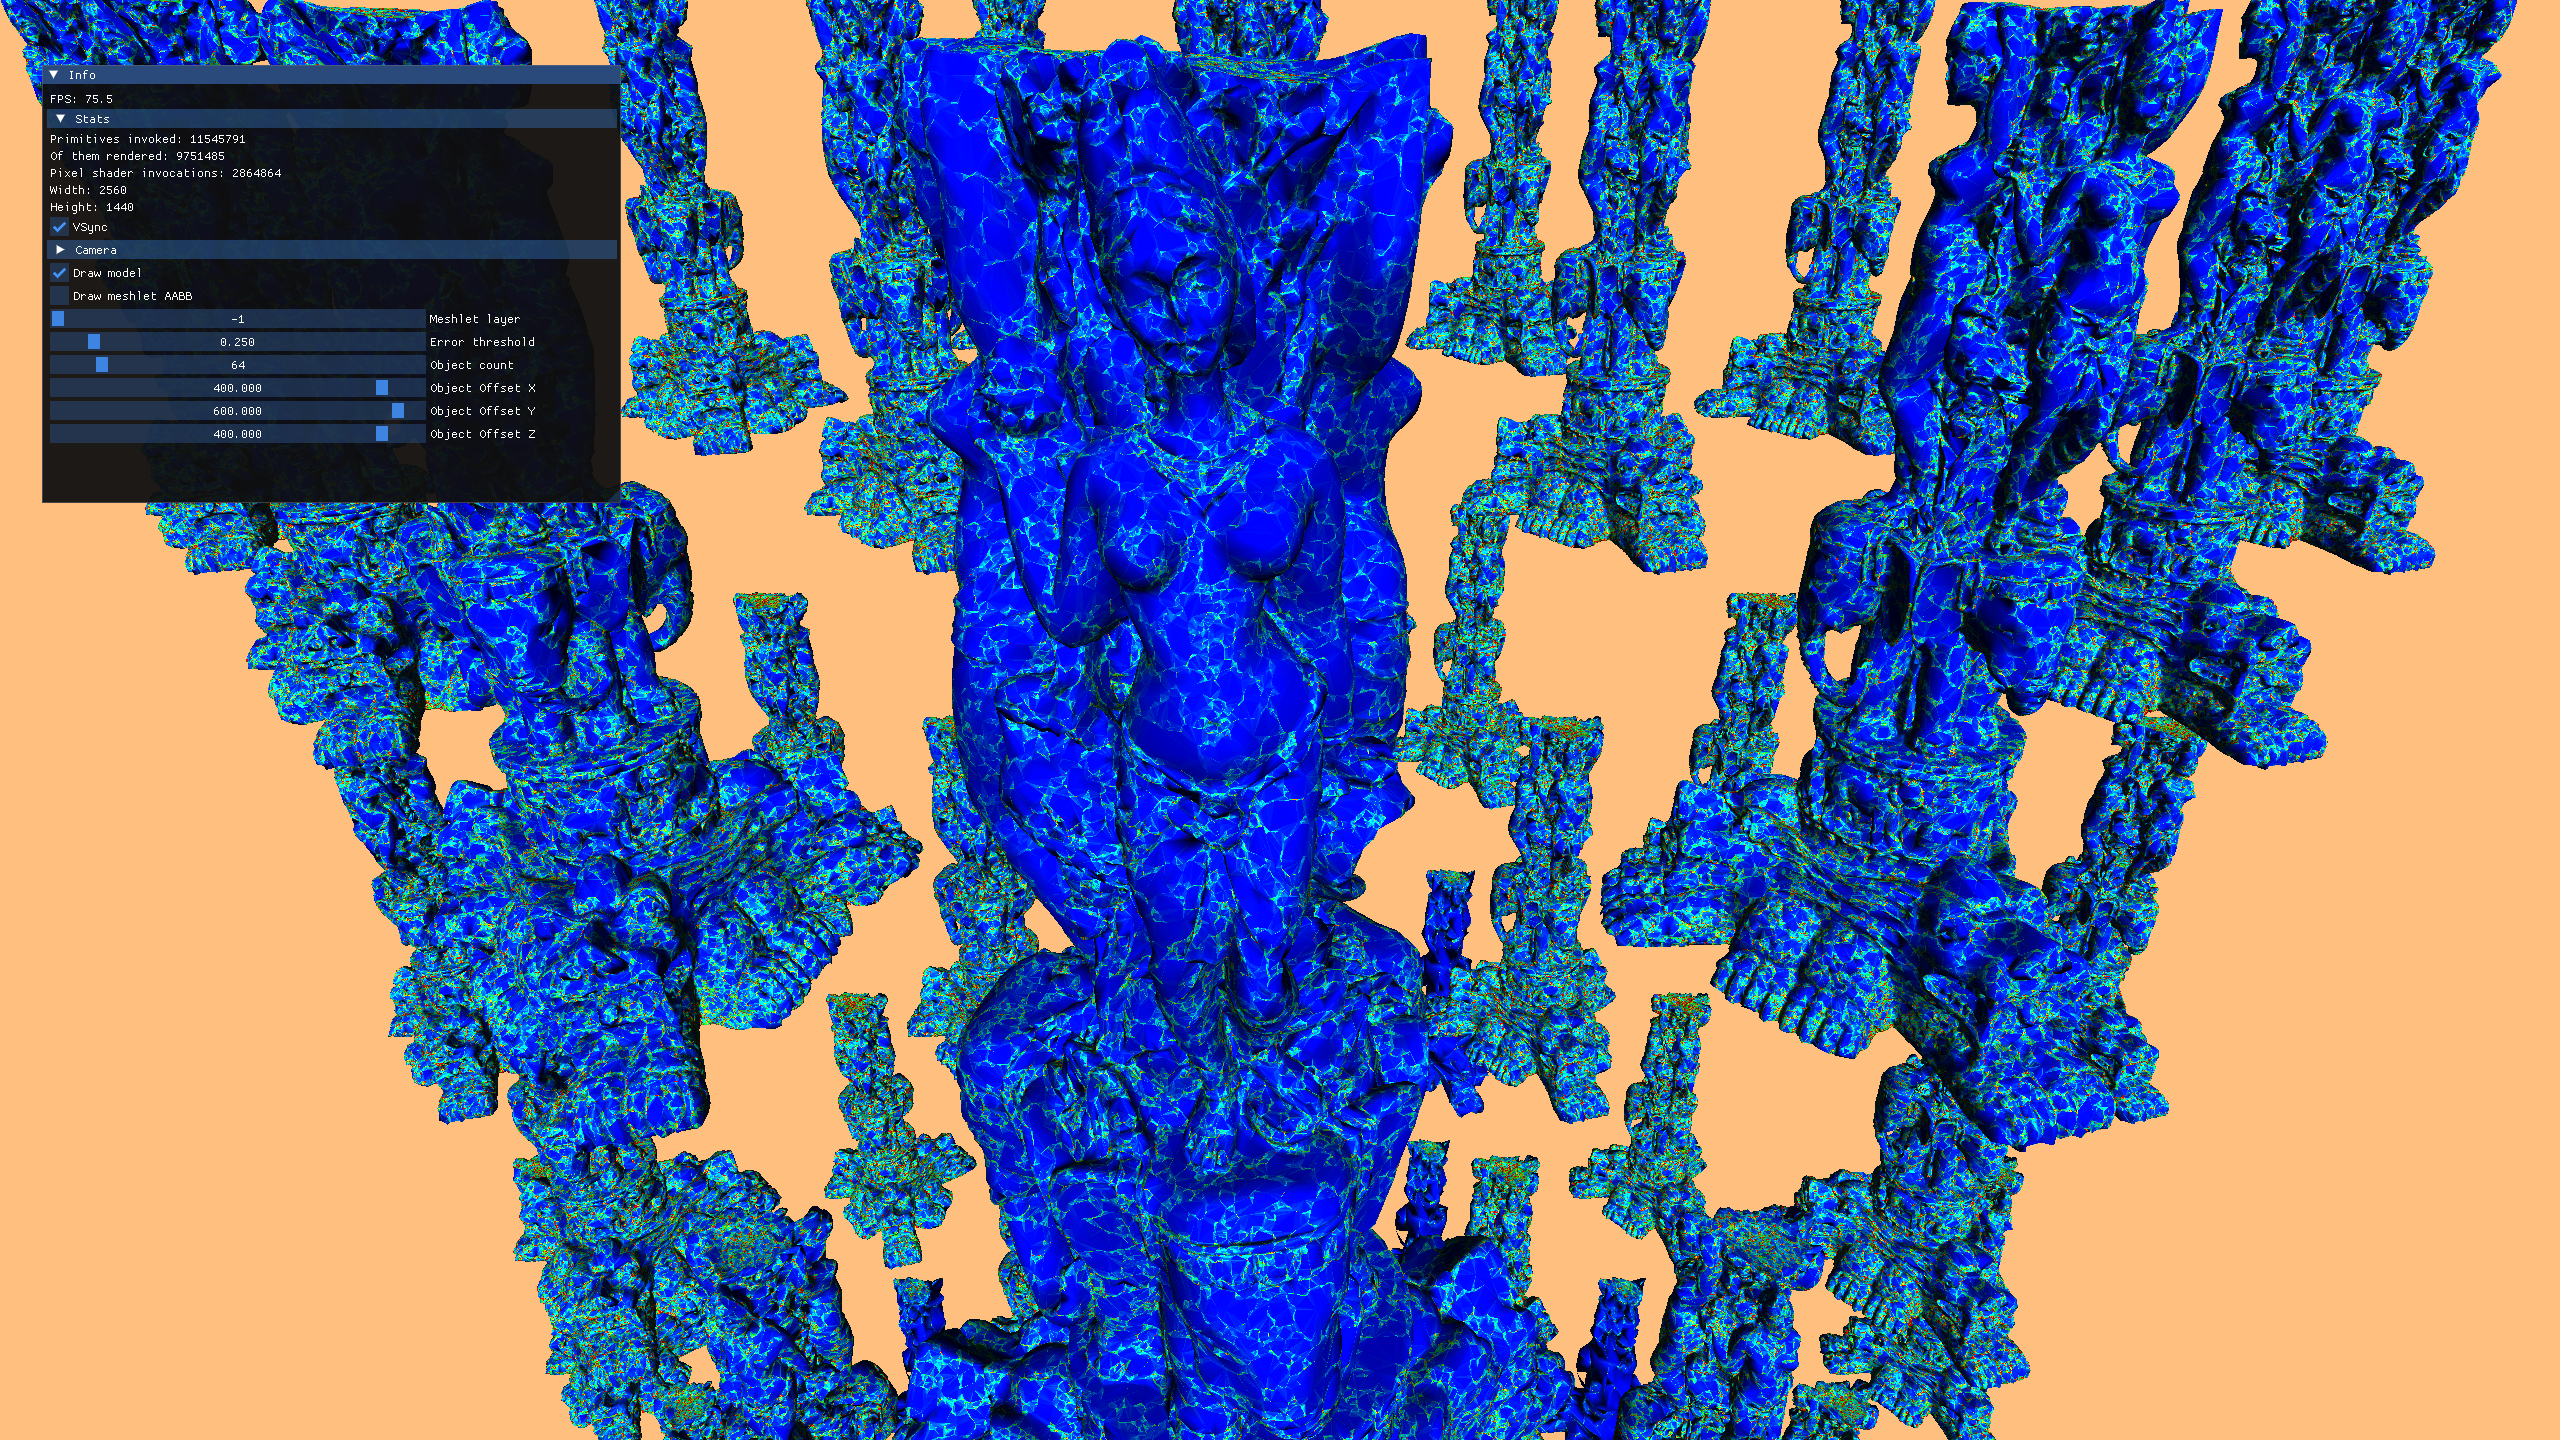
\includegraphics[width=\textwidth]{pics/impl-heatmap-cluster.png}
    \caption{Площадь треугольников мешлетов}
    \label{fig:impl-heatmap-cluster}
\end{figure}

\begin{figure}[H]
    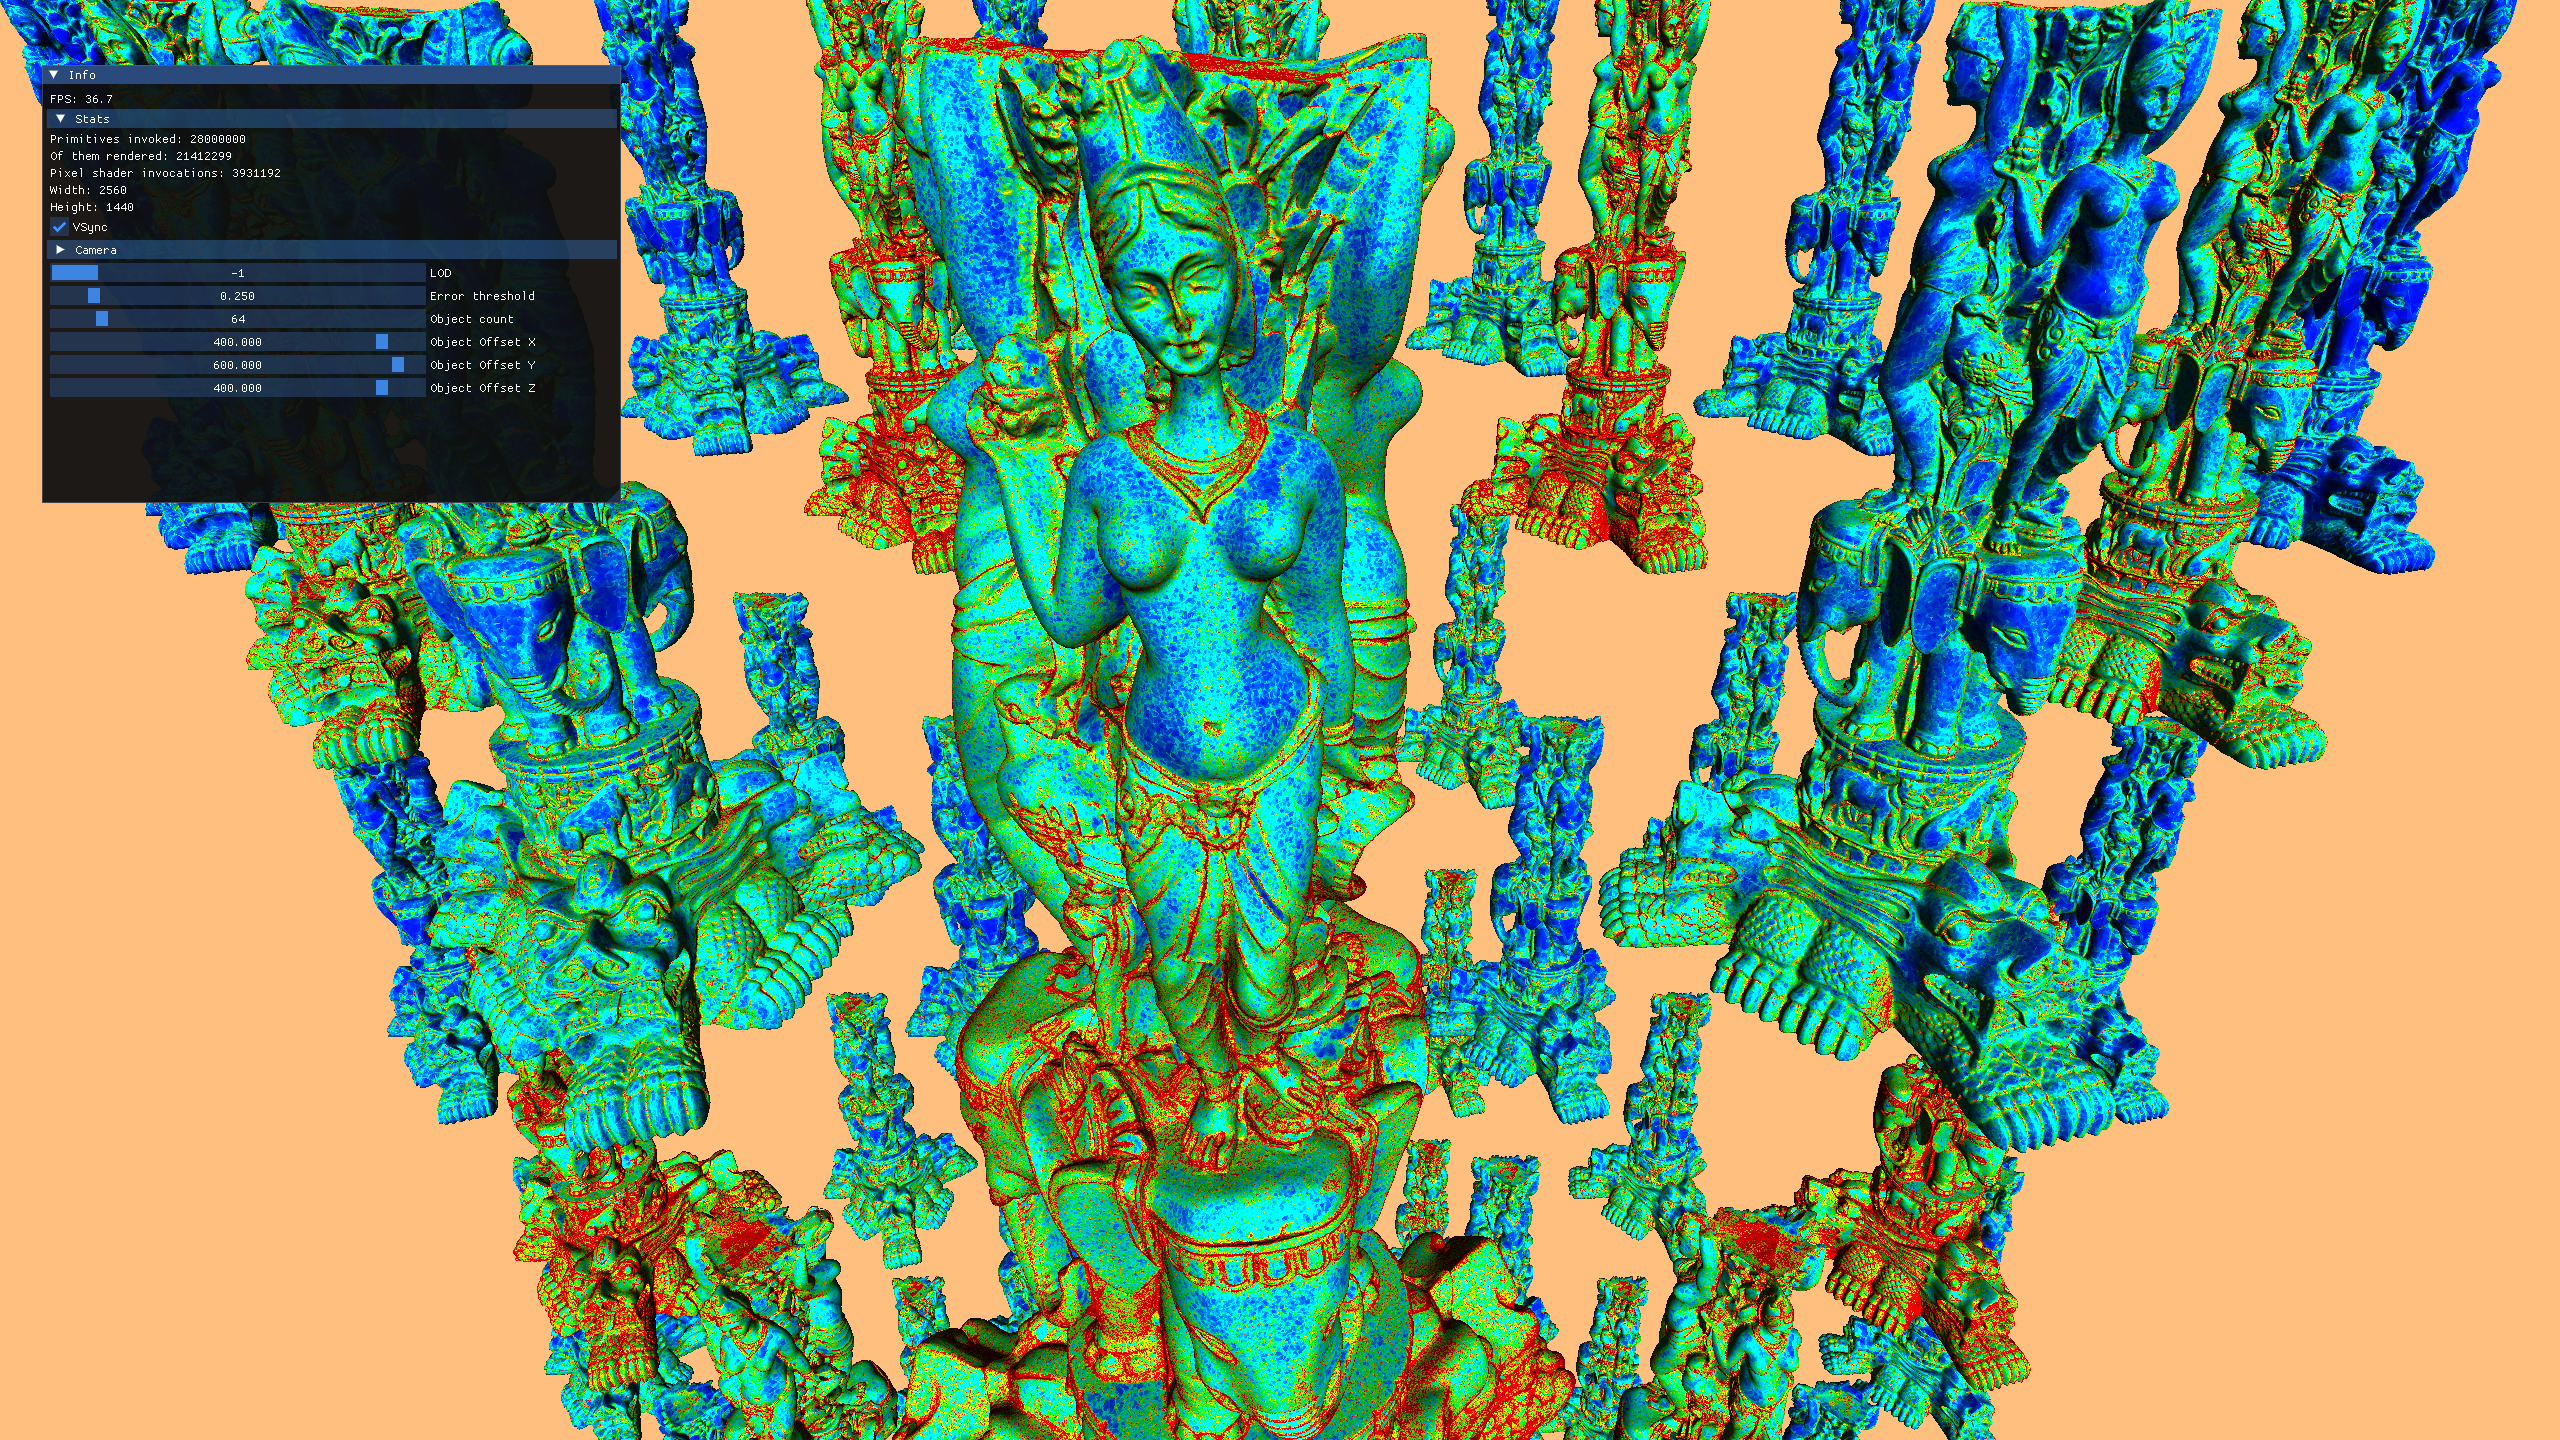
\includegraphics[width=\textwidth]{pics/impl-heatmap-mono.png}
    \caption{Площадь треугольников лодов}
    \label{fig:impl-heatmap-mono}
\end{figure}

Рисунки~\ref{fig:impl-heatmap-cluster} и~\ref{fig:impl-heatmap-mono} показывают, что с помощью кластерных лодов удалось добиться более равномерной площади проекций треугольников, чем с помощью монолитных лодов.
При этом концентрация малых треугольников на большом удалении от камеры показывает, что оценка, на основании которой производится выбор, пока недостаточно точна, и нужно искать способы её улучшить.

\subsection*{Заключение главы}
Сравнение с тривиальным алгоритмом монолитного лоддирования показало, что полученная реализация технологии процедурного кластерного видозависимого лоддирования пока сущетсвенно проигрывает в производительности, достигая только 31\% частоты кадров.
Для исправления этого в дальнейших работах предлагается исследовать те оптимизации, предложенные в главе 3, которые не были реализованы в данной работе.
